\documentclass[a4paper,10pt]{article}
\usepackage[utf8]{inputenc}
\usepackage[margin=2cm]{geometry}
\usepackage{tikz}
\usetikzlibrary{shapes.geometric, arrows.meta, positioning, matrix, fit, backgrounds, calc}
\usepackage{amsmath}

\definecolor{blue1}{RGB}{33,150,243}
\definecolor{orange1}{RGB}{255,152,0}
\definecolor{green1}{RGB}{76,175,80}
\definecolor{red1}{RGB}{244,67,54}
\definecolor{lightblue}{RGB}{144,202,249}
\definecolor{lightorange}{RGB}{255,224,178}
\definecolor{lightgreen}{RGB}{200,230,201}
\definecolor{gray1}{RGB}{28,28,28}
\definecolor{darkgray}{RGB}{66,66,66}

\pagestyle{empty}

\begin{document}

\begin{center}
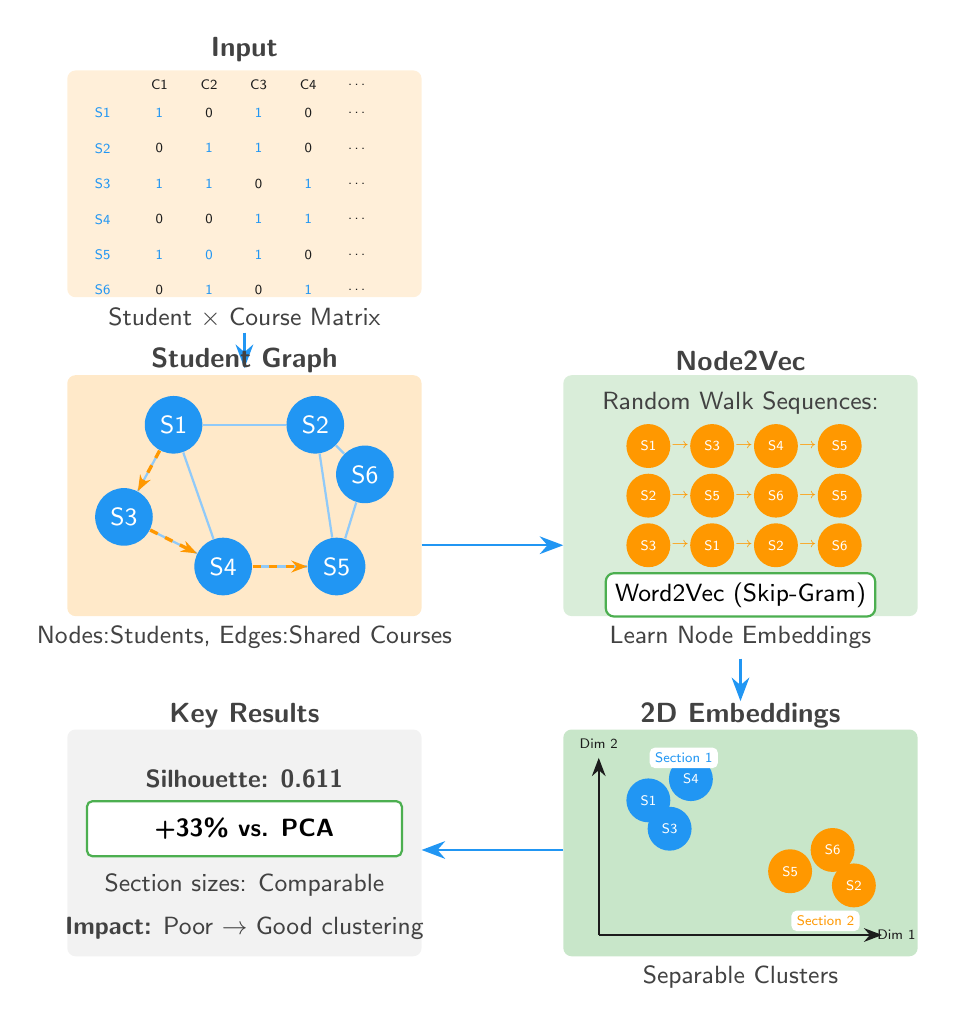
\begin{tikzpicture}[
    node distance=0.8cm,
    scale=0.9,
    every node/.style={font=\sffamily}
]

% ============================================================
% STAGE 1: Student-Course Matrix (Top)
% ============================================================
\node[font=\sffamily\bfseries, text=darkgray] at (-4.5, 12.5) {Input};

% Matrix background
\fill[lightorange!50, rounded corners=3pt] (-7, 9.0) rectangle (-2, 12.2);

% Students
\node[font=\sffamily\tiny, text=blue1] at (-6.5, 11.6) {S1};
\node[font=\sffamily\tiny, text=blue1] at (-6.5, 11.1) {S2};
\node[font=\sffamily\tiny, text=blue1] at (-6.5, 10.6) {S3};
\node[font=\sffamily\tiny, text=blue1] at (-6.5, 10.1) {S4};
\node[font=\sffamily\tiny, text=blue1] at (-6.5, 9.6) {S5};
\node[font=\sffamily\tiny, text=blue1] at (-6.5, 9.1) {S6};

% Course labels
\node[font=\sffamily\tiny, text=gray1] at (-5.7, 12.0) {C1};
\node[font=\sffamily\tiny, text=gray1] at (-5.0, 12.0) {C2};
\node[font=\sffamily\tiny, text=gray1] at (-4.3, 12.0) {C3};
\node[font=\sffamily\tiny, text=gray1] at (-3.6, 12.0) {C4};
\node[font=\sffamily\tiny, text=gray1] at (-2.9, 12.0) {\dots};

% Matrix entries
\node[font=\sffamily\tiny, text=blue1] at (-5.7, 11.6) {1};
\node[font=\sffamily\tiny, text=gray1] at (-5.0, 11.6) {0};
\node[font=\sffamily\tiny, text=blue1] at (-4.3, 11.6) {1};
\node[font=\sffamily\tiny, text=gray1] at (-3.6, 11.6) {0};
\node[font=\sffamily\tiny, text=gray1] at (-2.9, 11.6) {\dots};

\node[font=\sffamily\tiny, text=gray1] at (-5.7, 11.1) {0};
\node[font=\sffamily\tiny, text=blue1] at (-5.0, 11.1) {1};
\node[font=\sffamily\tiny, text=blue1] at (-4.3, 11.1) {1};
\node[font=\sffamily\tiny, text=gray1] at (-3.6, 11.1) {0};
\node[font=\sffamily\tiny, text=gray1] at (-2.9, 11.1) {\dots};

\node[font=\sffamily\tiny, text=blue1] at (-5.7, 10.6) {1};
\node[font=\sffamily\tiny, text=blue1] at (-5.0, 10.6) {1};
\node[font=\sffamily\tiny, text=gray1] at (-4.3, 10.6) {0};
\node[font=\sffamily\tiny, text=blue1] at (-3.6, 10.6) {1};
\node[font=\sffamily\tiny, text=gray1] at (-2.9, 10.6) {\dots};

\node[font=\sffamily\tiny, text=gray1] at (-5.7, 10.1) {0};
\node[font=\sffamily\tiny, text=gray1] at (-5.0, 10.1) {0};
\node[font=\sffamily\tiny, text=blue1] at (-4.3, 10.1) {1};
\node[font=\sffamily\tiny, text=blue1] at (-3.6, 10.1) {1};
\node[font=\sffamily\tiny, text=gray1] at (-2.9, 10.1) {\dots};

\node[font=\sffamily\tiny, text=blue1] at (-5.7, 9.6) {1};
\node[font=\sffamily\tiny, text=blue1] at (-5.0, 9.6) {0};
\node[font=\sffamily\tiny, text=blue1] at (-4.3, 9.6) {1};
\node[font=\sffamily\tiny, text=gray1] at (-3.6, 9.6) {0};
\node[font=\sffamily\tiny, text=gray1] at (-2.9, 9.6) {\dots};

\node[font=\sffamily\tiny, text=gray1] at (-5.7, 9.1) {0};
\node[font=\sffamily\tiny, text=blue1] at (-5.0, 9.1) {1};
\node[font=\sffamily\tiny, text=gray1] at (-4.3, 9.1) {0};
\node[font=\sffamily\tiny, text=blue1] at (-3.6, 9.1) {1};
\node[font=\sffamily\tiny, text=gray1] at (-2.9, 9.1) {\dots};

\node[font=\sffamily\small, text=darkgray] at (-4.5, 8.7) {Student $\times$ Course Matrix};

% Arrow down
\draw[-{Stealth[length=3mm]}, blue1, thick] (-4.5, 8.5) -- (-4.5, 8.0);

% ============================================================
% STAGE 2: Student Graph (Middle Left)
% ============================================================
\node[font=\sffamily\bfseries, text=darkgray] at (-4.5, 8.1) {Student Graph};

% Graph background
\fill[lightorange!70, rounded corners=3pt] (-7, 4.5) rectangle (-2, 7.9);

% Nodes
\node[circle, fill=blue1, text=white, minimum size=0.6cm, font=\sffamily\small] (s1) at (-5.5, 7.2) {S1};
\node[circle, fill=blue1, text=white, minimum size=0.6cm, font=\sffamily\small] (s2) at (-3.5, 7.2) {S2};
\node[circle, fill=blue1, text=white, minimum size=0.6cm, font=\sffamily\small] (s3) at (-6.2, 5.9) {S3};
\node[circle, fill=blue1, text=white, minimum size=0.6cm, font=\sffamily\small] (s4) at (-4.8, 5.2) {S4};
\node[circle, fill=blue1, text=white, minimum size=0.6cm, font=\sffamily\small] (s5) at (-3.2, 5.2) {S5};
\node[circle, fill=blue1, text=white, minimum size=0.6cm, font=\sffamily\small] (s6) at (-2.8, 6.5) {S6};

% Edges
\draw[lightblue, thick] (s1) -- (s2);
\draw[lightblue, thick] (s1) -- (s3);
\draw[lightblue, thick] (s1) -- (s4);
\draw[lightblue, thick] (s2) -- (s5);
\draw[lightblue, thick] (s2) -- (s6);
\draw[lightblue, thick] (s3) -- (s4);
\draw[lightblue, thick] (s4) -- (s5);
\draw[lightblue, thick] (s5) -- (s6);

% Random walk path
\draw[-{Stealth[length=2mm]}, orange1, very thick, dashed] (s1) -- (s3);
\draw[-{Stealth[length=2mm]}, orange1, very thick, dashed] (s3) -- (s4);
\draw[-{Stealth[length=2mm]}, orange1, very thick, dashed] (s4) -- (s5);

\node[font=\sffamily\small, text=darkgray] at (-4.5, 4.2) {Nodes:Students, Edges:Shared Courses};

% Arrow to Node2Vec
\draw[-{Stealth[length=3mm]}, blue1, thick] (-2.0, 5.5) -- (0.0, 5.5);

% ============================================================
% STAGE 3: Random Walks + Word2Vec (Middle Right)
% ============================================================
\node[font=\sffamily\bfseries, text=darkgray] at (2.5, 8.1) {Node2Vec};

% Node2Vec background
\fill[lightgreen!70, rounded corners=3pt] (0, 4.5) rectangle (5, 7.9);

% Walk sequences
\node[font=\sffamily\small, text=darkgray, align=left] at (2.5, 7.5) {Random Walk Sequences:};

% Walk 1
\node[circle, fill=orange1, text=white, minimum size=0.35cm, font=\sffamily\tiny] at (1.2, 6.9) {S1};
\node[font=\sffamily\tiny, text=orange1] at (1.65, 6.9) {$\rightarrow$};
\node[circle, fill=orange1, text=white, minimum size=0.35cm, font=\sffamily\tiny] at (2.1, 6.9) {S3};
\node[font=\sffamily\tiny, text=orange1] at (2.55, 6.9) {$\rightarrow$};
\node[circle, fill=orange1, text=white, minimum size=0.35cm, font=\sffamily\tiny] at (3.0, 6.9) {S4};
\node[font=\sffamily\tiny, text=orange1] at (3.45, 6.9) {$\rightarrow$};
\node[circle, fill=orange1, text=white, minimum size=0.35cm, font=\sffamily\tiny] at (3.9, 6.9) {S5};

% Walk 2
\node[circle, fill=orange1, text=white, minimum size=0.35cm, font=\sffamily\tiny] at (1.2, 6.2) {S2};
\node[font=\sffamily\tiny, text=orange1] at (1.65, 6.2) {$\rightarrow$};
\node[circle, fill=orange1, text=white, minimum size=0.35cm, font=\sffamily\tiny] at (2.1, 6.2) {S5};
\node[font=\sffamily\tiny, text=orange1] at (2.55, 6.2) {$\rightarrow$};
\node[circle, fill=orange1, text=white, minimum size=0.35cm, font=\sffamily\tiny] at (3.0, 6.2) {S6};
\node[font=\sffamily\tiny, text=orange1] at (3.45, 6.2) {$\rightarrow$};
\node[circle, fill=orange1, text=white, minimum size=0.35cm, font=\sffamily\tiny] at (3.9, 6.2) {S5};

% Walk 3
\node[circle, fill=orange1, text=white, minimum size=0.35cm, font=\sffamily\tiny] at (1.2, 5.5) {S3};
\node[font=\sffamily\tiny, text=orange1] at (1.65, 5.5) {$\rightarrow$};
\node[circle, fill=orange1, text=white, minimum size=0.35cm, font=\sffamily\tiny] at (2.1, 5.5) {S1};
\node[font=\sffamily\tiny, text=orange1] at (2.55, 5.5) {$\rightarrow$};
\node[circle, fill=orange1, text=white, minimum size=0.35cm, font=\sffamily\tiny] at (3.0, 5.5) {S2};
\node[font=\sffamily\tiny, text=orange1] at (3.45, 5.5) {$\rightarrow$};
\node[circle, fill=orange1, text=white, minimum size=0.35cm, font=\sffamily\tiny] at (3.9, 5.5) {S6};

% Word2Vec box
\node[draw=green1, thick, rounded corners=3pt, fill=white, minimum width=2cm, minimum height=0.5cm, font=\sffamily\small] at (2.5, 4.8) {Word2Vec (Skip-Gram)};

\node[font=\sffamily\small, text=darkgray] at (2.5, 4.2) {Learn Node Embeddings};

% Arrow to 2D Embeddings
\draw[-{Stealth[length=3mm]}, blue1, thick] (2.5, 3.9) -- (2.5, 3.3);

% ============================================================
% STAGE 4: 2D Embedding Space (Bottom Right)
% ============================================================
\node[font=\sffamily\bfseries, text=darkgray] at (2.5, 3.1) {2D Embeddings};

% Embedding space background
\fill[lightgreen, rounded corners=3pt] (0, -0.3) rectangle (5, 2.9);

% Axes
\draw[-{Stealth}, gray1, thick] (0.5, 0) -- (0.5, 2.5);
\draw[-{Stealth}, gray1, thick] (0.5, 0) -- (4.5, 0);

\node[font=\sffamily\tiny, text=gray1] at (0.5, 2.7) {Dim 2};
\node[font=\sffamily\tiny, text=gray1] at (4.7, 0) {Dim 1};

% Cluster 1 (blue)
\node[circle, fill=blue1, text=white, minimum size=0.4cm, font=\sffamily\tiny] at (1.2, 1.9) {S1};
\node[circle, fill=blue1, text=white, minimum size=0.4cm, font=\sffamily\tiny] at (1.8, 2.2) {S4};
\node[circle, fill=blue1, text=white, minimum size=0.4cm, font=\sffamily\tiny] at (1.5, 1.5) {S3};

% Cluster 2 (orange)
\node[circle, fill=orange1, text=white, minimum size=0.4cm, font=\sffamily\tiny] at (3.2, 0.9) {S5};
\node[circle, fill=orange1, text=white, minimum size=0.4cm, font=\sffamily\tiny] at (3.8, 1.2) {S6};
\node[circle, fill=orange1, text=white, minimum size=0.4cm, font=\sffamily\tiny] at (4.1, 0.7) {S2};

% Cluster labels
\node[font=\sffamily\tiny, text=blue1, fill=white, rounded corners=2pt, inner sep=2pt] at (1.7, 2.5) {Section 1};
\node[font=\sffamily\tiny, text=orange1, fill=white, rounded corners=2pt, inner sep=2pt] at (3.7, 0.2) {Section 2};

\node[font=\sffamily\small, text=darkgray] at (2.5, -0.6) {Separable Clusters};

% Arrow to Results
\draw[-{Stealth[length=3mm]}, blue1, thick] (0.0, 1.2) -- (-2.0, 1.2);

% ============================================================
% STAGE 5: Improved Clustering Results (Bottom Left)
% ============================================================
\node[font=\sffamily\bfseries, text=darkgray] at (-4.5, 3.1) {Key Results};

% Results background
\fill[gray!10, rounded corners=3pt] (-7, -0.3) rectangle (-2, 2.9);

% Result metrics
\node[font=\sffamily\small, text=darkgray, align=left] at (-4.5, 2.2) {\textbf{Silhouette: 0.611}};

\node[draw=green1, thick, rounded corners=2pt, fill=white, minimum width=4cm, minimum height=0.7cm, font=\sffamily\small] at (-4.5, 1.5) {\textbf{+33\% vs. PCA}};

\node[font=\sffamily\small, text=darkgray, align=left] at (-4.5, 0.7) {Section sizes: Comparable};

% Impact
\node[font=\sffamily\small, text=darkgray, align=left] at (-4.5, 0.1) {\textbf{Impact:} Poor $\rightarrow$ Good clustering};

\end{tikzpicture}
\end{center}

\end{document}